\begin{figure}[t]
\centering
  \subfigure[$\gls{G}_0$]{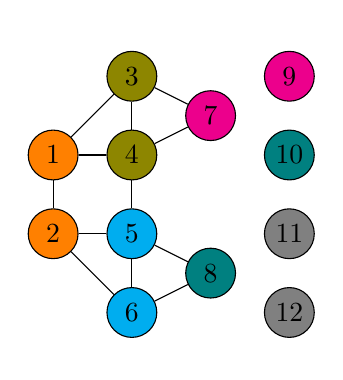
\begin{tikzpicture}
  \fill [white] (-1, -2) rectangle (1, 2) node {};  % Zentriere Graph.
  \tikzstyle{node}=[circle,draw, minimum width=18pt, inner sep=0pt, fill=white]
  \tikzstyle{color1}=[fill=orange]
  \tikzstyle{color2}=[fill=olive]
  \tikzstyle{color3}=[fill=cyan]
  \tikzstyle{color4}=[fill=magenta]
  \tikzstyle{color5}=[fill=teal]
  \tikzstyle{color6}=[fill=gray]

  \node[node, color1] (1)  at (-2, 0.5)  {$1$};
  \node[node, color1] (2)  at (-2, -0.5) {$2$};
  \node[node, color2] (3)  at (-1, 1.5)  {$3$};
  \node[node, color2] (4)  at (-1, 0.5)  {$4$};
  \node[node, color3] (5)  at (-1, -0.5) {$5$};
  \node[node, color3] (6)  at (-1, -1.5) {$6$};
  \node[node, color4] (7)  at (0,  1)    {$7$};
  \node[node, color5] (8)  at (0,  -1)   {$8$};

  \node[node, color4] (9)  at (1, 1.5)   {$9$};
  \node[node, color5] (10) at (1, 0.5)   {$10$};
  \node[node, color6] (11) at (1, -0.5)  {$11$};
  \node[node, color6] (12) at (1, -1.5)  {$12$};

  \path (1) edge (2);
  \path (1) edge (3);
  \path (1) edge (4);
  \path (2) edge (5);
  \path (2) edge (6);
  \path (3) edge (4);
  \path (3) edge (7);
  \path (4) edge (5);
  \path (4) edge (7);
  \path (5) edge (6);
  \path (5) edge (8);
  \path (6) edge (8);
\end{tikzpicture}
}
\hspace{1cm}
  \subfigure[$\gls{G}_1$]{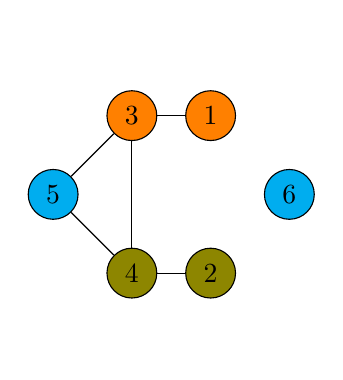
\begin{tikzpicture}
  \fill [white] (-1, -2) rectangle (1, 2) node {};  % Zentriere Graph.
  \tikzstyle{node}=[circle,draw, minimum width=18pt, inner sep=0pt, fill=white]
  \tikzstyle{color1}=[fill=orange]
  \tikzstyle{color2}=[fill=olive]
  \tikzstyle{color3}=[fill=cyan]

  \node[node, color3] (1) at (-1, 0) {$5$};
  \node[node, color1] (2) at (0,  1) {$3$};
  \node[node, color2] (3) at (0, -1) {$4$};
  \node[node, color1] (4) at (1,  1) {$1$};
  \node[node, color2] (5) at (1, -1) {$2$};

  \node[node, color3] (6) at (2, 0)  {$6$};

  \path (1) edge (2);
  \path (1) edge (3);
  \path (2) edge (3);
  \path (2) edge (4);
  \path (3) edge (5);
\end{tikzpicture}
}
\hspace{1cm}
  \subfigure[$\gls{G}_2$]{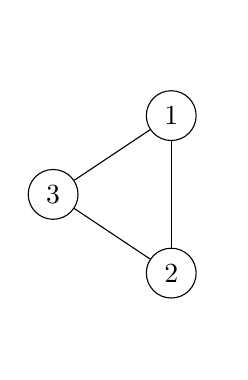
\begin{tikzpicture}
  \fill [white] (-1, -2) rectangle (1, 2) node {};  % Zentriere Graph.
  \tikzstyle{node}=[circle,draw, minimum width=18pt, inner sep=0pt, fill=white]

  \node[node] (1) at (-1,   0) {$3$};
  \node[node] (2) at (0.5,  1) {$1$};
  \node[node] (3) at (0.5, -1) {$2$};

  \path (1) edge (2);
  \path (1) edge (3);
  \path (2) edge (3);
\end{tikzpicture}
}
\hspace{1cm}
  \subfigure[Anorderung der Knoten zu einem binären Baum]{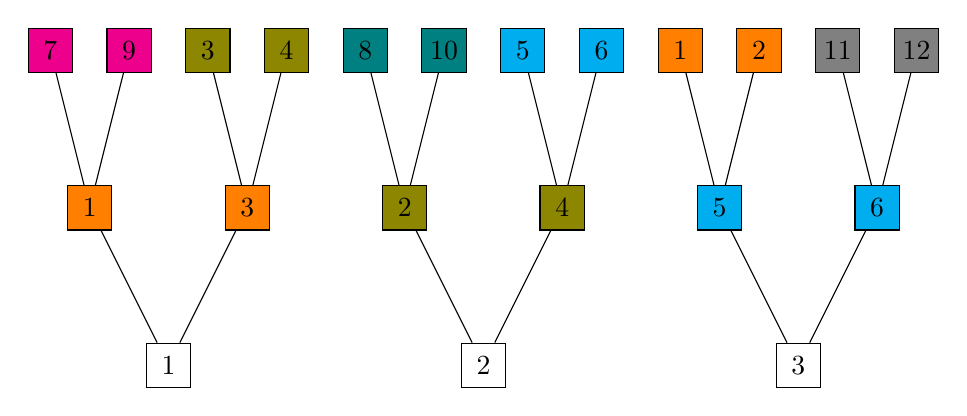
\begin{tikzpicture}
  \tikzstyle{node}=[rectangle,draw, minimum width=16pt, minimum height=16pt, inner sep=0pt, fill=white]
  \tikzstyle{color1}=[fill=orange]
  \tikzstyle{color2}=[fill=olive]
  \tikzstyle{color3}=[fill=cyan]
  \tikzstyle{color4}=[fill=magenta]
  \tikzstyle{color5}=[fill=teal]
  \tikzstyle{color6}=[fill=gray]

  \node[node, color4] (01)  at (-5.5, 2) {$7$};
  \node[node, color4] (02)  at (-4.5, 2) {$9$};
  \node[node, color2] (03)  at (-3.5, 2) {$3$};
  \node[node, color2] (04)  at (-2.5, 2) {$4$};
  \node[node, color5] (05)  at (-1.5, 2) {$8$};
  \node[node, color5] (06)  at (-0.5, 2) {$10$};
  \node[node, color3] (07)  at (0.5,  2) {$5$};
  \node[node, color3] (08)  at (1.5,  2) {$6$};
  \node[node, color1] (09)  at (2.5,  2) {$1$};
  \node[node, color1] (010) at (3.5,  2) {$2$};
  \node[node, color6] (011) at (4.5,  2) {$11$};
  \node[node, color6] (012) at (5.5,  2) {$12$};

  \node[node, color1] (11) at (-5, 0) {$1$};
  \node[node, color1] (12) at (-3, 0) {$3$};
  \node[node, color2] (13) at (-1, 0) {$2$};
  \node[node, color2] (14) at (1,  0) {$4$};
  \node[node, color3] (15) at (3,  0) {$5$};
  \node[node, color3] (16) at (5,  0) {$6$};

  \node[node] (21) at (-4, -2)  {$1$};
  \node[node] (22) at (0,  -2)  {$2$};
  \node[node] (23) at (4,  -2)  {$3$};

  \path (21) edge (11);
  \path (21) edge (12);
  \path (22) edge (13);
  \path (22) edge (14);
  \path (23) edge (15);
  \path (23) edge (16);
  \path (11) edge (01);
  \path (11) edge (02);
  \path (12) edge (03);
  \path (12) edge (04);
  \path (13) edge (05);
  \path (13) edge (06);
  \path (14) edge (07);
  \path (14) edge (08);
  \path (15) edge (09);
  \path (15) edge (010);
  \path (16) edge (011);
  \path (16) edge (012);
\end{tikzpicture}
}
\caption[Pooling auf Graphen]{Illustration einer Pooling-Operationen der Größe $4$ (\bzw{} zweier Pooling-Operationen der Größe $2$) auf einem Graphen \gls{G} der Größe $\left|\gls{V}\right| = 8$.
Das Clustering von \gls{G} liefert uns im ersten Schritt $N_1 =\left|\gls{V}_1\right| = 5$ Knoten und im darauf folgenden $N_2 = \left|\gls{V}_2\right| = 3$ Knoten.
Die Größen der Graphen werden daraufhin zu $N_2 = 3$, $N_1 = 6$ und $N_0 = 12$ angepasst, so dass jeder Knoten auf genau $2$ Vorgängerknoten verweist, indem \enquote{Fake}-Knoten zu $\gls{G}_1$ (1 Knoten) und $\gls{G}_0$ (4 Knoten) hinzugefügt werden.
Mit der Anordnung der Knoten zu einem binären Baum (d) kann die Pooling-Operation $\max\left(\cdot\right)$ eines Signals $\ve{f} \in \gls{R}^{12}$ auf $\gls{G}_0$ dann effizient als $\ve{f}_{\mathrm{pool}} \coloneqq {\left[ \max\left(\ve{f}_1, \ve{f}_2, \ve{f}_3, \ve{f}_4 \right), \max\left(\ve{f}_5, \ve{f}_6, \ve{f}_7, \ve{f}_8 \right), \max\left(\ve{f}_9, \ve{f}_{10}, \ve{f}_{11}, \ve{f}_{12} \right) \right]}^{\top} \in \gls{R}^3$ implementiert werden, wobei die Werte der \enquote{Fake}-Knoten $\ve{f}_2, \ve{f}_6, \ve{f}_{11}, \ve{f}_{12}$ auf den neutralen Wert $0$ gesetzt werden.}
\label{fig:pooling}
\end{figure}
